\documentclass[12pt]{article}
\usepackage{amsmath, amssymb}  % Add useful math symbols and environments
\usepackage{amsfonts}          % Add fonts for sets like \mathbb{Z}
\usepackage{enumitem}          % Better control of list formatting
\usepackage[amsthm,thmmarks]{ntheorem} %Proof formatting
\newcommand{\Z}{\mathbb{Z}}    % Custom command for integers
\newcommand{\sset}{\subseteq}  % Custom command for subset notation
\usepackage{graphicx}
\usepackage{tikz}
\usepackage[dvipsnames]{xcolor}

\begin{document}

\begin{center}
	{\LARGE Discrete Math - Homework 7} \Large \newline
    Name:
    % Write your name here.
\end{center}

\noindent \emph{Instruction summary:} Your work must be uploaded to Gradescope as a single PDF file. It must be typed in LaTeX to avoid a 20\% penalty. The polished proof must start in a new page (\textbackslash{newpage}). It will be graded based on clarity, LaTeX prowess and proof quality (including, for example, structure and variable definition).

%------------------------------
% EXERCISES
%------------------------------
\section*{Exercises:}

\begin{enumerate}

% QUESTION 1
\item \emph{(3 points)} Let \( a, b \in \mathbb{R} \). Define a sequence \( (u_n) \) by giving \( u_0, u_1 \), and for all \( n \in \mathbb{N} \),
\[
u_{n+2} = a u_{n+1} + b u_n.
\]
Prove by strong induction that for all \( n \in \mathbb{N} \),
\[
u_n = \alpha r_1^n + \beta r_2^n,
\]
with \( r_1^2 = a r_1 + b \), \( r_2^2 = a r_2 + b \); and where \( \alpha \) and \( \beta \) are the solutions to the system
\[
\left\{
\begin{array}{rcll}
u_0 & = & \alpha + \beta & \text{(n=0)} \\
u_1 &= & \alpha r_1 + \beta r_2 & \text{(n=1)}
\end{array}
\right.
\]

\emph{Hint: You are not proving \( u_{n+2} = a u_{n+1} + b u_n \) but instead \( u_n = \alpha r_1^n + \beta r_2^n \). You will need to use \( r_1^2 = a r_1 + b \) and \( r_2^2 = a r_2 + b \) at some point during the induction step.} \newline

% Write your answers to question 1 here.

% QUESTION 2
\item \emph{(3 points)} Let \( a, b \in \mathbb{R} \). Define a sequence \( (u_n) \) by giving \( u_0, u_1 \), and for all \( n \in \mathbb{N} \),
\[
u_{n+2} = a u_{n+1} + b u_n.
\]
Prove by strong induction that for all \( n \in \mathbb{N} \),
\[
u_n = \alpha r_0^n + \beta n r_0^n,
\]
with \( r_0^2 = a r_0 + b \) and \( a = 2r_0 \); and where \( \alpha \) and \( \beta \) are the solutions to the system
\[
\left\{
\begin{array}{rcl}
  \alpha & = & u_0 \\
  \alpha r_0 + \beta r_0 & = & u_1
\end{array}
\right.
\] \newline

% Write your answers to question 2 here.


% QUESTION 3
\item \emph{(4 points)} Fix \( b \in \mathbb{N} \).

\begin{enumerate}
\item Show by induction that for all \( n \in \mathbb{N} \),
\[
\sum_{k = 0}^n \binom{k+b}{k} = \binom{n + b + 1}{b+1}.
\]
\emph{Hint: Remember that for \( 0 < k \leq n \)} 
\[
\binom{n}{k} = \binom{n}{n-k} \hspace{1cm} \hspace{1cm} 
\]
\emph{and the Pascal's identity}
\[
\binom{n+1}{k} = \binom{n}{k} + \binom{n}{k-1}  \hspace{1cm} \hspace{1cm} 
\] \newline

% Write your answers to question 3a here.

\item Give a combinatorial proof of this identity. \newline

% Write your answers to question 3b here.

\end{enumerate}

% QUESTION 4
\item \emph{(5 points)} We have a rectangular grid with \( b+1 \) nodes high (\( b \) rows) and \( a+1 \) nodes on the base (\( a \) columns) with \( a, b \in \mathbb{N} \). Also \( a \in \{ b, b+1 \} \), so there is one grid associated with each value of \( n = a + b \). 

We want to go from the bottom-left node to the top-right node. The only moves allowed are either going to the node immediately above or to the right. 
How many different paths are there for a given value of \( n \)? The solutions for \( n \leq 4 \) are plotted below:

\begin{center} %% This is tikz. All of the code below is to draw the figure. Don't change any of it!
    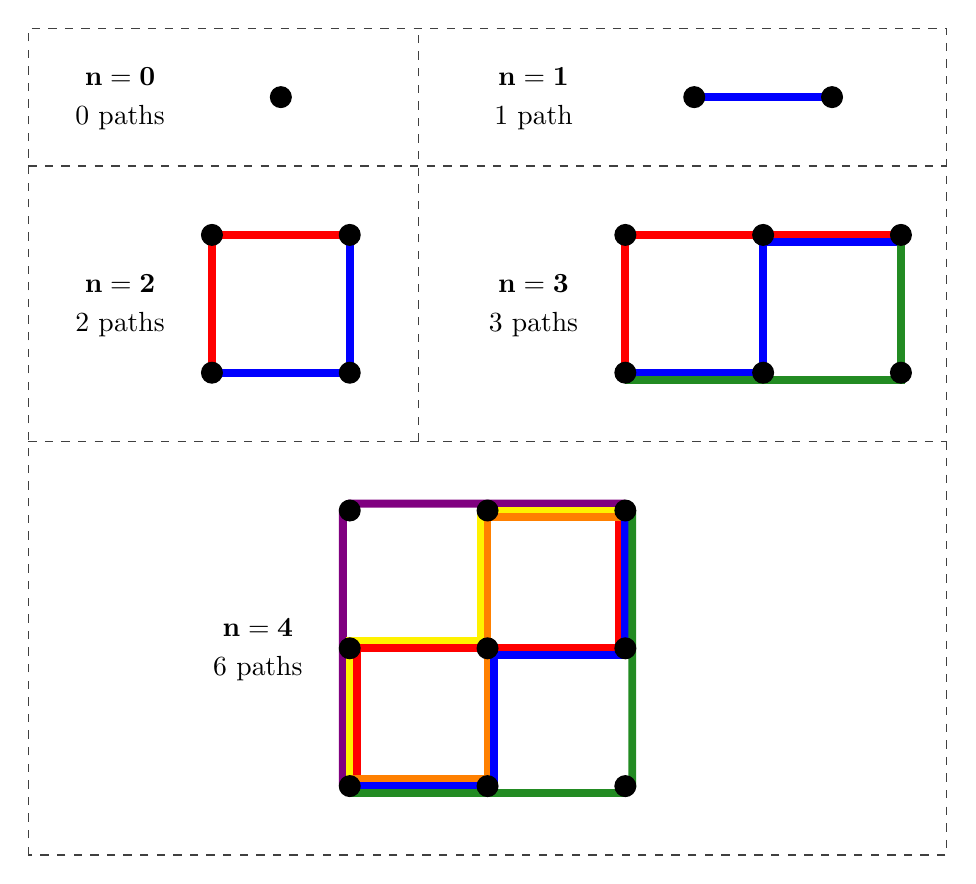
\begin{tikzpicture}[scale=1.75]
        \draw[black!75!white,dashed] (-4/3,-3.5) -- (-4/3,2.5) -- (16/3,2.5) -- (16/3,-3.5) -- (-4/3,-3.5);
        \draw[black!75!white,dashed] (-4/3,1.5) -- (16/3,1.5); \draw[black!75!white,dashed] (-4/3,-0.5) -- (16/3,-0.5);
        \draw[black!75!white,dashed] (1.5,-0.5) -- (1.5,2.5);
    
        \draw (-2/3,2.15) node {$\mathbf{n=0}$}; \draw (-2/3,1.85) node {$0$ paths}; 
        \foreach\x in {0}{\foreach\y in {0}{\filldraw ({\x+0.5},{\y+2}) circle(.5ex);}}
        
        \draw (-2/3,0.65) node {$\mathbf{n=2}$}; \draw (-2/3,0.35) node {$2$ paths}; 
        \draw[line width=1mm,red] (0,0) -- (0,1) -- (1,1); 
        \draw[line width=1mm,blue] (0,0) -- (1,0) -- (1,1);
        \foreach\x in {0,1}{\foreach\y in {0,1}{\filldraw ({\x},{\y}) circle(.5ex);}}
        
        \draw (7/3,2.15) node {$\mathbf{n=1}$}; \draw (7/3,1.85) node {$1$ path}; 
        \draw[line width=1mm,blue] (3.5,2) -- (4.5,2);
        \foreach\x in {0,1}{\foreach\y in {0}{\filldraw ({\x+3.5},{\y+2}) circle(.5ex);}}
        
        \draw (7/3,0.65) node {$\mathbf{n=3}$}; \draw (7/3,0.35) node {$3$ paths}; 
        \draw[line width=1mm,red] (3,0) -- (3,1) -- (5,1);
        \draw[line width=1mm,blue] (3,0) -- (4,0) -- (4,0.95) -- (5, 0.95) -- (5,1);
        \draw[line width=1mm,ForestGreen]   (3,-0.05) -- (5,-0.05) -- (5,1);
        \foreach\x in {0,1,2}{\foreach\y in {0,1}{\filldraw ({\x+3},{\y}) circle(.5ex);}}
        
        \draw ({19/3-6},{1.15-3}) node {$\mathbf{n=4}$}; \draw ({19/3-6},{0.85-3}) node {$6$ paths};
        \draw[line width=1mm,violet] (0.95,-3) -- (0.95,-1) -- (1,-0.95) -- (3,-0.95); 
        \draw[line width=1mm,yellow] (1,-3) -- (1,-1.95) -- (1.95,-1.95) -- (1.95,-1) -- (3,-1); 
        \draw[line width=1mm,red] (1.05,-3) -- (1.05,-2) -- (2.95,-2) -- (2.95,-1);
        \draw[line width=1mm,orange] (1,-2.95) -- (2,-2.95) -- (2,-1.05) -- (3,-1.05); 
        \draw[line width=1mm,blue] (1,-3) -- (2.05,-3) -- (2.05,-2.05) -- (3,-2.05) -- (3,-1);
        \draw[line width=1mm,ForestGreen] (1,-3.05) -- (3,-3.05) -- (3.05,-3) -- (3.05,-1);
        \foreach\x in {0,1,2}{\foreach\y in {0,1,2}{\filldraw ({\x+1},{\y-3}) circle(.5ex);}}
    \end{tikzpicture}
\end{center}

From these examples, we think we may have figured out a property. For \( n \in \mathbb{N} \), define the property \( \mathcal{P}(n) \): ``If a grid has \( a \) columns and \( b \) rows with \( a + b = n \), then the number of paths from bottom-left to top-right in this grid is \( \binom{a+b}{a} \).''

Prove this property by induction.

\emph{Hint: The upper right node can be accessed either from the node to the left or from the node right below.} \newline

% Write your answers to question 4 here.


\end{enumerate}
\newpage %Please do not erase this line.

%------------------------------
% POLISHED PROOF
%------------------------------
\section*{Polished proof:} 

\emph{(10 points)} Consider two numbers \( a, b \in \mathbb{R} \), and the sequence \( (u_n) \) obtained by successively taking the average of the last two numbers in the sequence, starting with \( a \) and \( b \). 

Thus, by definition, we have \( u_0 = a \), \( u_1 = b \), and for all \( n \in \mathbb{N} \),
\[
u_{n+2} = \frac12 \left( u_{n+1} + u_n \right).
\]
For instance, if \( a = 1 \) and \( b = 4 \), you get
\[
u_0 = 1, \quad u_1 = 4, \quad u_2 = \frac{5}{2}, \quad u_3 = \frac{13}{4}, \quad \dots
\]

Prove by induction that for all \( n \in \mathbb{N} \) we have
\[
u_n = \frac{1}{3} ( a + 2b) + \frac{2}{3} (a - b) \left( - \frac{1}{2} \right)^n.
\]
Please mark with a little title each part of the proof.



\noindent \emph{Claim.}
% Write here the statement you intent to prove. E.g: "Claim: There is only one even prime number."

\begin{proof}
%Write your proof here.
\end{proof}


\end{document}